\documentclass[]{article}
\usepackage{listings}
\usepackage{graphicx}
\usepackage{float}
 
\floatstyle{ruled}
\newfloat{program}{thp}{lop}
\floatname{program}{Snippet}


\begin{document}

\title{Visualizing Software Projects in JavaScript}
\author{Tim Disney}
\date{}

\maketitle

\lstset{showstringspaces=false}

\begin{abstract}
  Visualization techniques have been used to help programmers deepen their understanding of large software projects. However the existing visualization techniques have focused on static languages where type information can only be determined at compile-time. This paper describes a new visualization tool aimed at the dynamic language JavaScript.
\end{abstract}

\section{Introduction}
\label{sec:introduction}
Programming is hard. As observed by Brooks \cite{brooks1987no} over 20 years ago there is an essential complexity to software that makes it so. Software developers spend much of their time managing the increasing complexities of their projects. Though there may be, as Brooks argues, no ``Silver Bullet'' to completely do away with all the painful complexity, there are techniques to alleviate at least some portion of the difficulty in building and understanding software projects. One technique has been the use of visualization tools. A number of tools have been created to help visualize the structure and relationships between packages and classes \cite{solidsx, haskellvis} and dependencies \cite{idea, stan4j} in software systems. Unfortunately these tools only work for static languages where the types in the system can be determined at compile-time. To the best of my knowledge there are no visualization tools for dynamic languages which create and mutate their objects at runtime.

This paper presents a visualization tool for JavaScript, a dynamic language used primarily in web browsers. This tool visualizes the structure of objects in a JavaScript application by using a node and link style graph. By capturing snapshots of the object structure at different points in the program execution, the visualization can display changes to the object structure at different points in time. 

This visualization tool allows developers to gain a deeper understanding of the structure of their application. This tool shows how objects are related, gives insight into object importance, and displays how structures change over the course of a running program. During development of this tool I was even able to discover a bug in a library by using the visualization.

This paper is structured as follows: section \ref{sec:background} gives an overview of JavaScript, section \ref{sec:method} describes how the visualization is created, section \ref{sec:results} describes the author's experiences using the tool, section \ref{sec:related} gives an overview of related work, section \ref{sec:future} describes possible future work and section \ref{sec:conclusion} concludes.

\section{Background}
\label{sec:background}
JavaScript \cite{ECMA-262} is a dynamic language primarily used in client-side web applications. Once regarded as a toy scripting language its popularity has increased in recent years due to its use in complex web applications such as Gmail and Google Maps.

JavaScript provides support for object oriented techniques but uses a prototype-based object system as opposed to the more traditional class-based system found in languages such as Java or C++. Objects in JavaScript are collections of mutable key/value properties roughly analogous to maps in Java or dictionaries in Python. The potential objects an application might use are not defined before instantiation, instead objects are instantiated and then mutated into their necessary form as the application executes.

When an object is created at the top level of a script (i.e. not locally scoped inside a function) it is added as a property to a global object (named {\tt window} in the browser environment). For example after the code in snippet \ref{snip:code} is executed the {\tt window} object will contain three properties: {\tt myObj} which is an object with properties {\tt foo} and {\tt baz}, {\tt myFun} which is a function, and {\tt globalVariable} which is the number 22. Each property can be referenced with the familiar dot notation (e.g. {\tt window.myObj.foo} gives ``bar'').

\begin{program}[here]
\begin{verbatim}
var myObj = {
  foo: "bar",
  baz: 42.34
};

function myFun(){
  var localVariable = 5;
  globalVariable = 22;
}
\end{verbatim}
\caption{Example JavaScript code}
\label{snip:code}
\end{program}

The reason {\tt globalVariable} is added to the global object is because it was not declared with the {\tt var} keyword. Any variable used in a function that has not been declared with {\tt var} is added to the global object. This is a source of potential bugs when developers forget to use {\tt var} since variable names might clash causing unexpected updates.

Since JavaScript does not have a module system to partition the namespace, it is standard practice for developers to use objects as a replacement. The Yahoo User Interface library (YUI) \cite{yui} is a good example of this. Every object used in YUI is contained in the top level {\tt YAHOO} object which is added to the global object. So for example if developers wish to use the calendar widget, they reference {\tt YAHOO.widget.Calendar}.

This use of objects as replacement modules provides a good place to begin visualization. Since most of the interesting objects in the system are available by traversing the global object, we can get an understanding of the project's structure by visualizing how these objects are related.

\section{Method}
\label{sec:method}
The visualization tool was written in JavaScript and runs in a web browser. The code is meant to be added to any JavaScript application that a user wishes to visualize. A user simply adds a script to their page and the visualization is displayed.


\begin{figure}[h]
  \begin{center}
    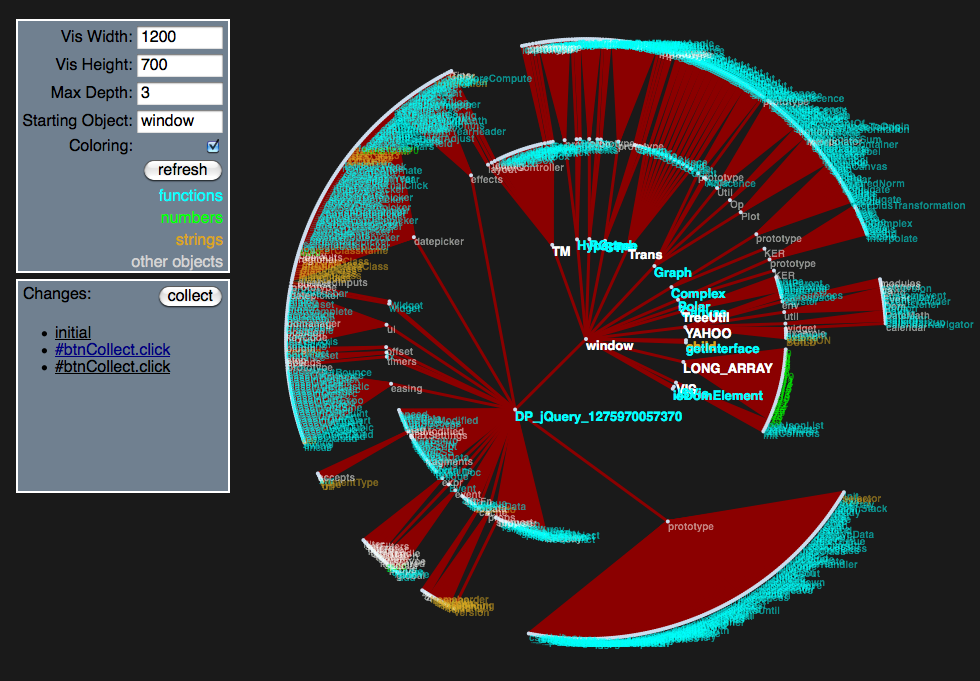
\includegraphics[scale=.35]{interface.png}
  \end{center}
  \caption{Global object three levels deep with interface}
  \label{fig:interface}
\end{figure}

To accomplish the visualization two main processes occur. First a process runs to collect the salient data. It accomplices this by starting with the global object {\tt window} and doing a depth-first search through each of its contained objects. As it walks each node (object) in the graph, it constructs a separate object with the data necessary to display the visualization. Essentially it is simplifying the object data so that it can be more easily translated into the visualization.

As this process is walking the object graph, it also does some filtering of the data. By default each browser provides a number of functions at the top level which are usually not very interesting to the developer since they are the same in every project. By default these are ignored. The collector process also does not traverse any DOM elements. These are the objects that represent the display elements in the browser window. Since the focus of the visualization is on the application and not the display, these are currently being ignored. It also ignores objects that have been previously visited to prevent creating circular references. This is a potential issue since it is sometimes useful to know that an object is referenced by multiple names. For example the jQuery library \cite{jquery} has two alias that can be used ({\tt \$} and {\tt jQuery}) and it is useful to know that both exist. Only the first name discovered by the collector is currently being displayed. Array are another special case in the collector. Since arrays are often used to hold large amounts of data (e.g. 1000s of elements) which is difficult to visualize, the collector will truncate arrays if they exceeded a set maximum number of elements (currently set at 30).



\begin{figure}[h]
  \begin{center}
    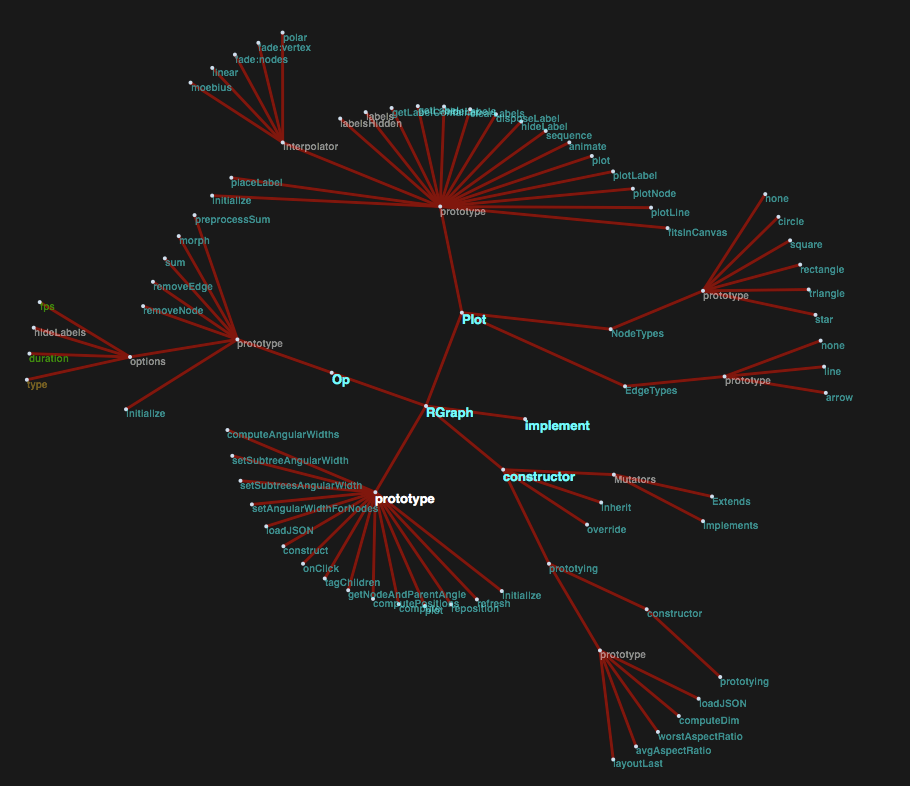
\includegraphics[scale=.35]{rgraph.png}
  \end{center}
  \caption{RGraph object four levels deep}
  \label{fig:rgraph}
\end{figure}

Once the simplified object has been created it is passed to a visualization library for display. The library being used is called the JavaScript InfoVis Toolkit (JIT) \cite{jit}. The specific visualization provided by JIT that is used is a radial tree inspired by the work done by Yee et al. \cite{yee2001animated}. The simplified object is transformed into a radial tree with each object represented as a node and lines between nodes representing contains relationships (see figure \ref{fig:interface}). Each node is colored to represent its type (blue for functions, green for numbers, orange for strings, and white for standard objects). 

Interactivity is provided by allowing a user to recenter the graph by clicking on a node. The user is also given controls to select the starting object (by default {\tt window}), maximum depth to traverse, size of the graph, and a toggle for node coloring. 

Since the data is collected at run-time, the visualization is able to collect the data multiple times and then display the changes between the graphs. There is a button in the interface to force collection to occur whenever a user clicks on it but the collection process can also be wired to any arbitrary events that can be triggered in the browser. Once the data has been collected the user can select a snapshot and the graph will morph into the new state recorded by that snapshot.


\section{Results}
\label{sec:results}

\begin{figure}[h]
  \begin{center}
    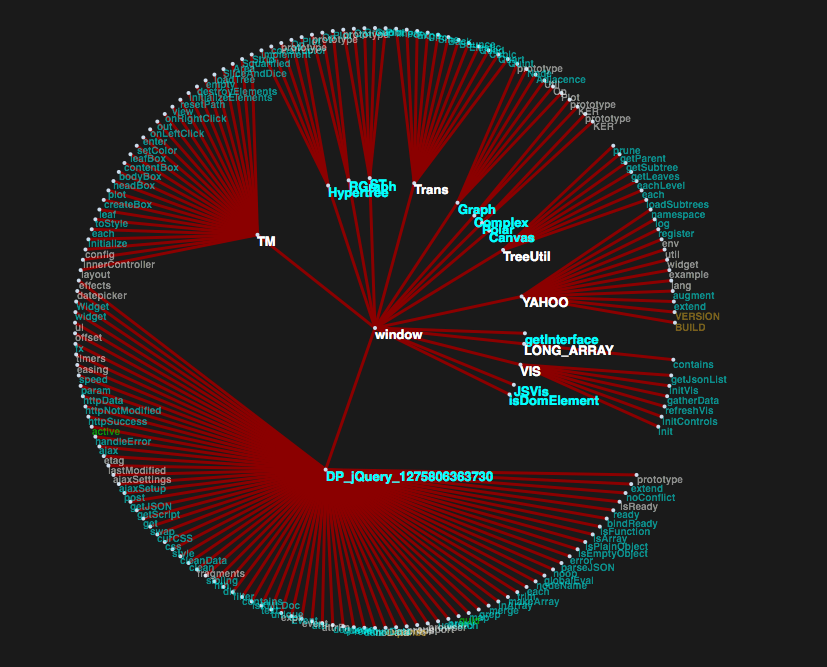
\includegraphics[scale=.35]{clean.png}
  \end{center}
  \caption{Clean Project}
  \label{fig:clean}
\end{figure}

While testing the visualization tool after it had been developed, I realized it would have been very useful during the development process. In particular I ran into difficulties trying to find a specific method on the JIT's RGraph object that would accomplish morphing the graph from one state to another. Though I eventually found the documentation for the necessary method, it was not obvious where it was located. If, instead of pouring through the documentation, I had looked at the graph of RGraph (seen in figure \ref{fig:rgraph}) the method, {\tt RGraph.op.prototype.morph}, would have been discovered much more rapidly.

During development I also managed to discover a programming flaw in the JIT visualization library. It appears that the programmers of JIT forgot to use the {\tt var} keyword when assigning to a variable called {\tt that}. I noticed this while testing out the change morphing, the {\tt that} variable showed up unexpectedly while moving from one change snapshot to another. Initially I thought that there was an error in my code but it quickly became obvious from the visualization that the values being stored in {\tt that} had to do with the internals of JIT.

\begin{figure}[h]
  \begin{center}
    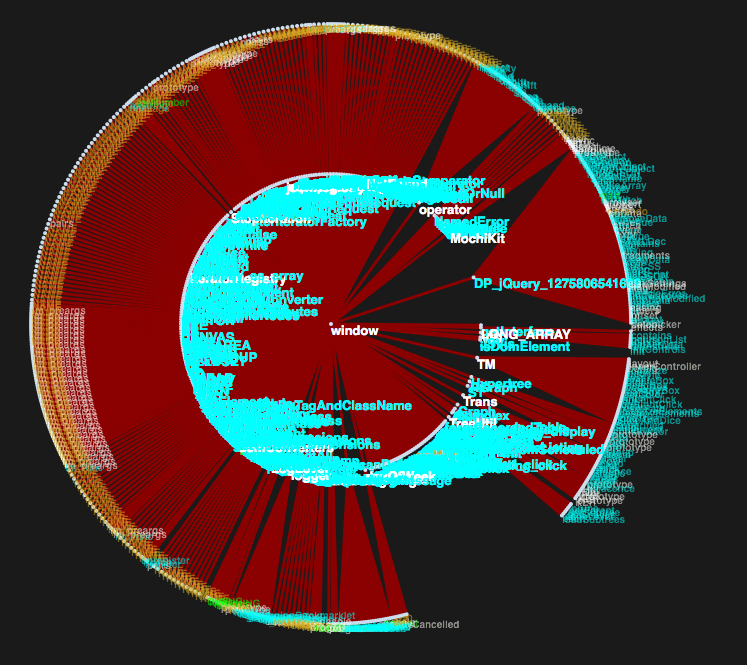
\includegraphics[scale=.38]{messy.png}
  \end{center}
  \caption{Messy Project}
  \label{fig:messy}
\end{figure}

Use of a variable called {\tt that} is actually a standard pattern in JavaScript development. It is commonly used to store a particular value of the {\tt this} object in a closure. Because the {\tt var} keyword was not used, the assignment to {\tt that} was placed on the global object. This is a potential source of bugs since multiple closures could possibly be in conflict over the contents of {\tt that}.


One of the goals of this visualization was to see the difference between a ``messy'' project and a ``clean'' project. Though the definitions are a bit fuzzy the intuition behind the terms is that a ``messy'' project has lots of objects in the global namespace while a ``clean'' project has relatively few. The reason for the value judgement in the terms is that when many objects are in the same namespace the chance for an unintentional conflict is greater resulting in subtle runtime bugs. Also with a ``clean'' project structure understandability and learning is facilitated. It is easier to find things when they have been grouped into hierarchies.


To see if the visualization would work well for visualizing the difference between a ``messy'' and ``clean'' project I ran the tool on two different projects. One was a project I had worked on several years ago when I was first learning how to program in JavaScript. The other was the use of a calendar widget from YUI. Although the comparison is partially unfair since the functionality of the two projects is very different, it does provide an illustrative example. As can be seen in the calendaring widget example in figure \ref{fig:clean} there are around half a dozen items in the top level with many more items under each of them. In contrast the old code base in figure \ref{fig:messy} has many items in the top level making it very difficult to make out one from the other.



%\begin{figure}[h]
%  \begin{center}
%    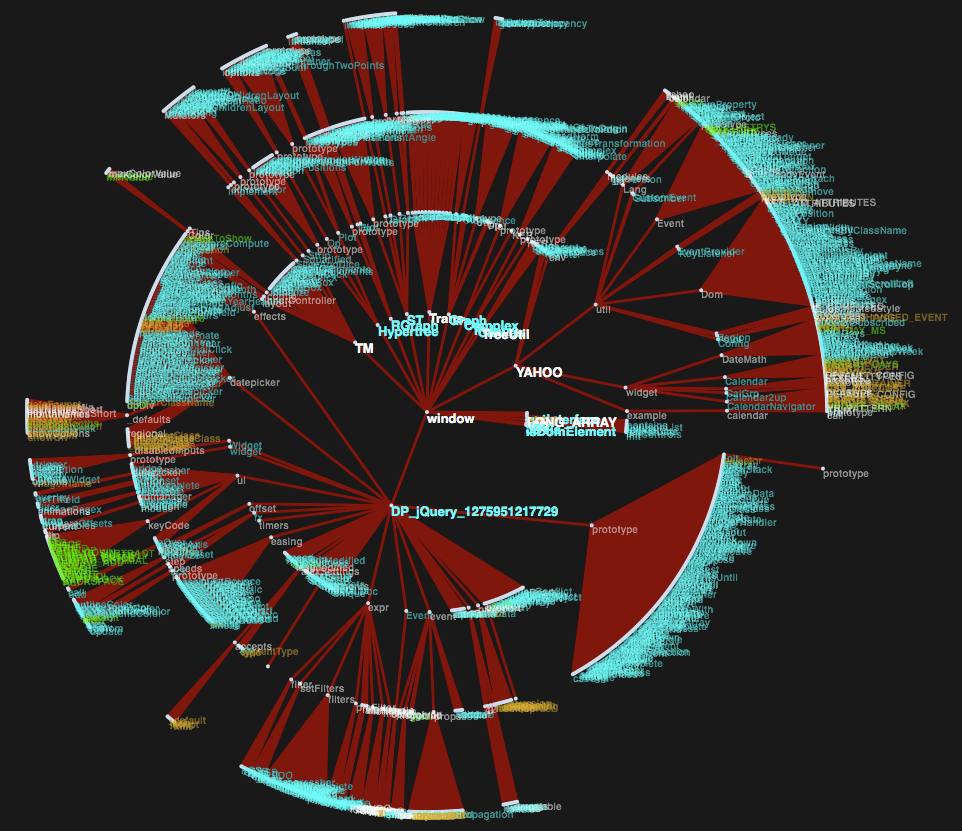
\includegraphics[scale=.2]{deep-window.png}
%  \end{center}
%  \caption{Global object four levels deep}
%  \label{fig:deep-window}
%\end{figure}


\begin{figure}[h]
  \begin{center}
    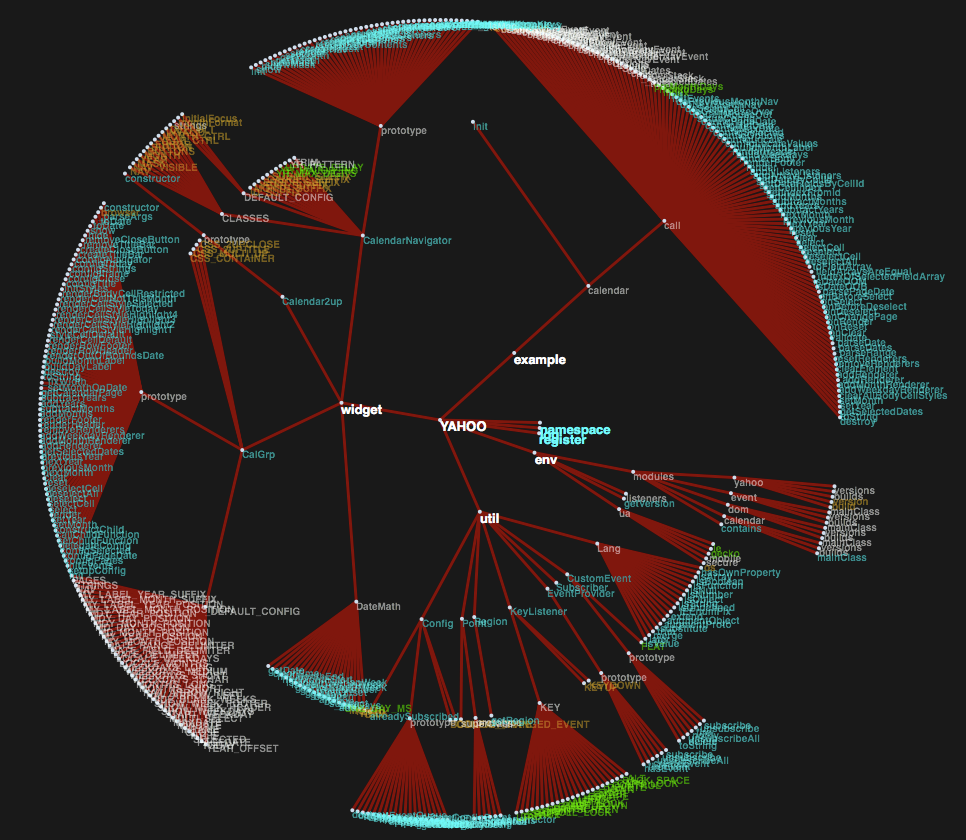
\includegraphics[scale=.35]{yahoo.png}
  \end{center}
  \caption{YAHOO object four levels deep}
  \label{fig:yahoo}
\end{figure}

\section{Related Work}
\label{sec:related}
There has been work on visualizing static languages. The commercial application SolidSX \cite{solidsx} runs on Java and .NET projects. There are IDE solutions built into IntelliJ IDEA \cite{idea} and available for Eclipse in the Stan4j project \cite{stan4j}. Don Stewart has published visualizations of Haskell code in the Hackage code repository \cite{haskellvis}.

There has also been work done on visualizing large hierarchies of data such as directory structures by Teoh et al. \cite{teoh2002rings, Wang2006} and Kleiberg \cite{kleiberg2001botanical}.

\section{Future Work}
\label{sec:future}
Currently the tool only collects object data available in the global object. This allows us to see many of the interesting object in the system however it does miss any objects scoped as function local variables. It would be interesting to see if adding this data would provide additional insights into the program structure.

Other potential work could include displaying all references to an object if more than one exists and user studies to determine how well this system works for other developers.

\section{Conclusion}
\label{sec:conclusion}
This paper has presented a visualization tool for the dynamic language JavaScript. It provides  deeper understanding of software projects, shows how objects are related, and gives insight into how object change over the course of a program.

\bibliographystyle{plain}
\bibliography{report}

\end{document}



